\Chapter{線形代数の広がり(佐藤)}
線形代数という分野は古いようで新しい.そもそも「線形代数(Linear Algebra)」という言葉が現代の意味で使われ始めたのは1930年に出版されたvan der Waerdenによる「現代代数学」という教科書の中でである.しかし線形代数における重要な概念はその教科書が出版されるずっと以前から少しずつ発明されていた.例えば,未知数の数と方程式の数が一致する場合の連立一次方程式の解法(Gaussの消去法)は、中国では「漢」の時代にはすでに発見されていたし,行列式にあたる概念はLeibnizや日本では関孝和\footnote{現在でいうところの終結式の概念を導入するために行列式を発見していたというのには驚きを隠せない.}が見つけていた.その後Sylvesterにより行列の概念が導入され,Cayley,Grassmann,Jordanなど19世紀に特に行列の理論についての研究が進んだ.私たちが現在大学初年級で習っている線形代数はそれらの結果を現代的に整備したものであり,抽象度が高く応用も広い反面,なぜそういったことを考えるのかというモチベーションがわかりにくくなっているように思う.この記事では,前半で行列や行列式の概念が多変数の微積分においてどのように出てくるのかを見た後,後半で抽象的な線形空間の例として多様体の接ベクトル空間というものを導入し,一つの応用として多様体上のベクトル場を挙げることにする.

\Section{多変数の微積分}
\Subsection{多変数における微分とは何か}
微分可能な1変数関数$f:\realnum\rightarrow\realnum$の$x=a$における「微分」(正確には微分係数)は$f'(a)$で与えられるのであった.このとき,Taylorの定理より,
$$
f(x)=f(a)+f'(a)(x-a)+o((x-a))
$$
が\footnote{以下,$o(x)$は$\lim_{x\rightarrow 0}\frac{o(x)}{x}=0$を満たすような項を表しているとする.}成り立つ.特に右辺の第2項は$f$の「1次近似」を与えていると考えることができ,$x=a$における$y=f(x)$のグラフをの接線の式は$y=f'(a)(x-a)+f(a)$となる.このように微分を関数の「1次近似」を与えるものとして考え,多変数に拡張してみる.


$n$変数の$C^1$級\footnote{各成分の偏導関数$\delxkf$が連続であること.}実数値関数$f:\realnum^n\rightarrow\realnum$と$\avec\in\realnum^n$が与えられているとする.多変数のTaylorの定理から
$$
f\xvec=f\avec+\sum_{k=1}^{n}\delxkf\avec(x_k-a_k)+o(\sqrt{(x_1-a_1)^2+\cdots+(x_n-a_n)^2})
$$
と$f$は表せる.1変数のときと同様に右辺の第2項に注目してみる.この部分は,$x={}^t\!(x_1,\dots,x_n), a={}^t\!(a_1,\dots,a_n), J=(\delxof(a_1,\dots,a_n) \dots \delxnf(a_1,\dots,a_n))$とおくと\footnote{紙面の節約のため縦ベクトル$\vecb x_1 \\ \vdots \\ x_n\vece$を${}^t\!(x_1,\dots,x_n)$と書く.}行列とベクトルの積$J(x-a)$と書けるから,上の式は
$$
f(x)=f(a)+J(x-a)+o(|x-a|)
$$
という非常にすっきりした形で表せる.特に,$x=a$における「接平面」の式は$y=J(x-a)+f(a)$となる.
さて,幾何学的に見れば,$\delxkf(a_1,\dots,a_n)$達はそれぞれ$(a_1,\dots,a_n)$における$e_k=\tenchi(0,\dots,1,\dots,0)$($k$番目の成分は1,それ以外は0)方向の変化率を表しているのだが,では一般に単位ベクトル$b=\tenchi(b_1,\dots,b_n)$方向の変化率はどう表せるだろうか.勿論極限の式から直接導くことは出来るが、ここでは接平面が$y=J(x-a)+f(a)$であることに注目すると,接平面における$b$方向の傾きは$Jb=\dsum_{k=1}^{n}\delxkf(a_1,\dots,a_n)b_k$であることから,$b$方向の$f$の変化率が$Jb$であることが簡単にわかる(もし$b$が単位ベクトルでない場合は$\dfrac{Jb}{|b|}$とあらわせる).このことから,$J$は$f$の$a$における全ての方向における1次近似の情報を持っていると見なせる.この$J$を上にならって$f$の$a$における「微分」と呼ぶことにしよう.


今までの議論は$f$の値域が$\realnum$,すなわち1次元の場合であった.もっと一般に$C^1$級写像$f:\realnum^n\rightarrow\realnum^m$が与えられたとする.結局値域が広がったところで,$m$個の$C^1$級関数$f_1,\dots,f_m$によって,$f\xvec=(f_1\xvec,\dots,f_m\xvec)$とあらわされるので,各$f_i:\realnum^n\rightarrow\realnum$について,1行$n$列の行列$J_i$が存在して,1次近似は$f_i(x)=f_i(a)+J_i(x-a)+o(|x-a|)$となる.この式を縦に並べて,$J=\vecb J_1\\ \vdots \\J_m\vece$という$m$行$n$列の行列を考えると,$f(x)=\tenchi(f_1(x),\dots,f_m(x)),f(a)=\tenchi(f_1(a),\dots,f_m(a))$と縦ベクトルで表せば,
$$
f(x)=f(a)+J(x-a)+o(|x-a|)
$$
という上と全く同じ式が得られる(ただし,この式は$m$次元ベクトルの等式なので,$o(|x-a|)$は各成分が$o(|x-a|)$であるようなベクトルを表していることに注意).上の式は特に$b\in\realnum^n$が十分小さいとき,$f(a+b)-f(a)\approx J(b)$と書けることを示していて,$f$によって$a$の$n$次元空間における「方向」が$f(a)$の$m$次元空間におけるどの「方向」に移るかを$J$は表していると考えられる.こうして多次元での微分を考える際には自然と行列の概念が出てくる.


$J$倍写像$\realnum^n\rightarrow\realnum^m$を「$n$次元方向」を「$m$次元方向」へ移す写像と考えたとき,$J$は次の性質をもつ.
\begin{description}
\item{(1)} 任意の$\lambda\in\realnum, x\in\realnum^n$に対して,$J(\lambda x)=\lambda J(x)$
\item{(2)} 任意の$x,y\in\realnum^n$に対して,$J(x+y)=J(x)+J(y)$
\end{description}
この性質によって,任意の$b=\tenchi(b_1,\dots,b_n)$に対して,$Jb=J(b_1e_1+\dots+ b_ne_n)=b_1J(e_1)+\dots+b_nJ(e_n)$となるが,$J$を成分によって明示的に表すと,
$$
J=\vecb \delxofo && \dots && \delxnfo \\ \vdots && && \vdots \\ \delxofm && \dots&&\delxnfm \\ \vece
$$
であるので,$J(e_k)=\tenchi\left(\delxkfo,\dots,\delxkfm\right)$となる.特に,$J$の各列ベクトルの線形結合によって,$Jb$は表される.すなわち,値域が$\realnum$から$\realnum^m$になっても$J$がすべての方向に関する1次近似の情報を持っていることには変わりがない.ところで,上の性質を満たすような$\realnum^n$から$\realnum^m$への写像は,ある行列$A$を用いて$A$倍写像とあらわされることが知られている.上の性質を満たすような写像を$\realnum^n$から$\realnum^m$への線形写像という.


まとめると,微分は$f:\realnum^n\rightarrow\realnum^m$の$a\in\realnum^n$における線形写像による近似を与えることと考えることが出来る.
このとき,この線形写像に対応する行列$J_f$をヤコビ行列という.ヤコビ行列の一つの応用として,微分の連鎖律を説明してみよう.
\begin{s_theo}[微分の連鎖律]
2つの$C^1$級写像$f:\realnum^n\rightarrow\realnum^m$と$g:\realnum^m\rightarrow\realnum^l$が与えられたとする.
このとき$J_{g\circ f}$で$a\in\realnum^n$における$g\circ f$のヤコビ行列
$J_f,J_g$で$f,g$の$a,f(a)$におけるヤコビ行列を表すと,
\[
J_{g\circ f}=J_gJ_f
\]
が成り立つ.
\end{s_theo}
\begin{Proof}
まず,$f,g$の1次近似は$f(a+b)-f(a)=J_f(b)+o(b),g(f(a)+b')-g(f(a))=J_g(b')+o(b')$と書けるから,$g(f(a+b))-g(f(a))=g(f(a)+f(a+b)-f(a))-g(f(a))=g(f(a)+J_f(b)+o(b))-g(f(a))=J_g(J_f(b)+o(b))+o(J_f(b)+o(b))=J_g(J_f(b))+o(b)$となる(最後の等号は,線形写像の性質(2)より$J_g(J_f(b)+o(b))=J_g(J_f(b))+J_g(o(b))$および,性質(1)と連続性より任意の線形写像$f$について,$f(o(x))=o(x),o(f(x))=o(x)$が成り立つことによる).よって,$g\circ f$の1次近似は$J_g$倍写像と$J_f$倍写像の合成で表される.ところで,行列の積の結合法則より,任意の$x\in\realnum^n$に対して$J_g(J_fx)=(J_gJ_f)x$が成り立つから,$J_g$倍写像と$J_f$倍写像の合成は$J_gJ_f$倍写像である.よって$J_{g\circ f}=J_gJ_f$となる.これが連鎖律とどう関係するかというと,両辺の成分を比べてみると,$\realnum^n$の変数を$x_1,\dots,x_n$,$\realnum^m$の変数を$y_1,\dots,y_m$として

$$
\vecb
\dfrac{\partial (g\circ f)_1}{\partial x_1}(a) && \dots && \dfrac{\partial (g\circ f)_1}{\partial x_n}(a) \\
\vdots                                           &&         && \vdots \\
\dfrac{\partial (g\circ f)_l}{\partial x_1}(a)  && \dots && \dfrac{\partial (g\circ f)_l}{\partial x_n}(a) \\
\vece
=
\vecb
\dfrac{\partial g_1}{\partial y_1}(f(a)) && \dots && \dfrac{\partial g_1}{\partial y_m}(f(a)) \\
\vdots                                           &&         && \vdots \\
\dfrac{\partial g_l}{\partial y_1}(f(a))  && \dots && \dfrac{\partial g_l}{\partial y_m}(f(a)) \\
\vece
\vecb
\dfrac{\partial f_1}{\partial x_1}(a) && \dots && \dfrac{\partial f_1}{\partial x_n}(a) \\
\vdots                                           &&         && \vdots \\
\dfrac{\partial f_m}{\partial x_1}(a)  && \dots && \dfrac{\partial f_m}{\partial x_n}(a) \\
\vece
$$
両辺の成分を比較して,$\dfrac{\partial (g\circ f)_i}{\partial x_j}(a)=\dsum_{k=1}^m\dfrac{\partial g_i}{\partial y_k}(f(a))\dfrac{\partial f_k}{\partial x_j}(a)$という等式を得る.
\end{Proof}

\Subsection{ヤコビ行列の応用と行列式}
前節においてヤコビ行列というものを導入したわけだが,ヤコビ行列は単なる1次近似の情報だけでなく,実は色々な情報を持っている.その例として逆関数定理と重積分の変数変換公式を紹介しよう.
\Subsubsection{逆関数定理}
まず,ヤコビ行列の行列式が$0$でないことはどういう情報であるかを表す\textbf{逆関数定理}について紹介する.
そのために,「開集合」という概念について説明しておく.「$\realnum^n$の部分集合$U$が$\realnum^n$の開集合である」とは,$U$の各点$x$に対して,十分小さい$\varepsilon>0$を取れば$x$から距離$\varepsilon$以内の点がすべて$U$に入るような集合のことを言う.直観的に言えば,開集合とは外部と接しているような点がないような集合のことで,例えば$\{(x,y)\in\realnum^2|x^2+y^2<1\}$は$\realnum^2$の開集合だが,$\{(x,y)\in\realnum^2|x^2+y^2\le1\}$はそうでない.$x\in\realnum^2$が入っているような$\realnum^n$の開集合のことを「$x$の$\realnum^n$における開近傍」という.ここで,$a\in\realnum^n$で微分するという操作は,$a$の十分近くで$f$が定義されていれば行えることに注意しよう(簡単な例として,$f(x)=\frac{1}{x}$は0以外のどこでも微分できるのであった).すると微分しようとする写像$f$は必ずしも$\realnum^n$全体で定義されている必要はなく,$a$の開近傍上で定義されていれば十分ということがわかる.準備が出来たところで逆関数定理のステートメントを述べよう.
\begin{s_theo}[逆関数定理]
$W$を$a\in\realnum^n$の$\realnum^n$における開近傍,$f:W\rightarrow\realnum^n$を$C^1$級写像とする.$a$における$f$のヤコビ行列$J_f$について,$J_f$の行列式$\det(J_f)$が0でないとき,$W$に含まれる$a$の$\realnum^n$におけるある開近傍$U$,$f(U)\subset V$をみたす$f(a)$の$\realnum^n$におけるある開近傍$V$,および$C^1$級写像$g:V\rightarrow U$が存在して,$f$の$U,V$への制限$\tilde{f}:U\rightarrow V$と$g$は互いに逆写像
\footnote{写像$p:A\rightarrow B$と$q:B\rightarrow A$が互いに逆写像とは,任意の$a\in A$に対して,$q(p(a))=a$および任意の$b\in B$に対して$p(q(b))=b$が成り立つことを言うのであった.}になっている.
\end{s_theo}
この定理は,\textbf{写像$f$の$a$におけるヤコビアンが$\det(J_f)$が$0$でなければ,$a$の周りで「局所的に」$f$はなめらかな逆写像を持つ,}ということを言っている.具体的に見てみよう.
\begin{figure}[h]
  \begin{center} 
    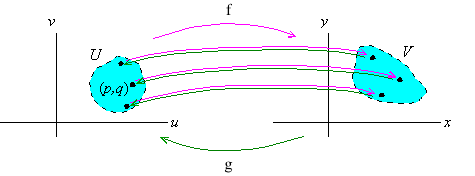
\includegraphics[width=7.0cm]{dev_invfunc}
    \caption{逆関数定理のイメージ}
  \end{center}
\end{figure}
\begin{s_ex}
$f:\realnum^2\rightarrow\realnum^2;(x,y)\mapsto(x+y,xy)$という写像を考えてみる.$f$は単射でも全射でもない.たとえば$f(2,1)=(3,2)=f(1,2)$であるし,$f(x,y)=(1,3)$を満たす$x,y\in\realnum$は存在しない.よって逆写像は存在しない.ここで,$(2,1)\in\realnum$においてヤコビ行列を計算してみると,
$$
\det(J_f)=\detb 1 && 1 \\ 1&& 2 \dete = 1\neq 0
$$
より,逆関数定理から,$(2,1)$の開近傍で逆写像をもつ.実際,$U=\{(x,y)\in\realnum^2|x>y\},V=\{(s,t)\in\realnum^2|s^2-4t>0\}$とおくと,$U$は$(2,1)$の$\realnum^2$における開近傍,$V$は$(3,2)$の$\realnum^2$における開近傍で$f(U)\subset V$であり,$C^1$級写像$g:V\rightarrow U$を$(s,t)\mapsto(\frac{s+\sqrt{s^2-4t}}{2},\frac{s-\sqrt{s^2-4t}}{2})$と定めると,$f$の制限$\tilde{f}:U\rightarrow V$と$g$は互いに逆写像となっている.
\end{s_ex}
この定理では$\det(J_f)\neq 0$という条件が一番本質的である.行列式の定義を思い出してみよう.$n$個の$\realnum^n$のベクトル$p_1,\dots,p_n$が与えられたとき,$P=(p_1\: p_2\dots p_n)$の行列式が0という条件は,$p_1,\dots,p_n$が一次従属であることと同値だった.直観的に言えば,$p_1,\dots,p_n$で張られる$n$次元平行四辺形の体積が潰れていなければ,$\det(P)\neq 0$となる.これを使って定理の直観的な説明を与えよう.$f$が仮定を満たすとする.$J_f$は$a$における線形近似を表していたので,$\lambda>0$が十分0に近ければ,$A=\{a+(x_1e_1+\dots+x_ne_n)\in\realnum^n|各kについて|x_k|<\lambda\}$という$a$を含む微小長方形内では,$f$は$J_f$が表す線形写像で近似でき,その像は$B=\{f(a)+(x_1J_f(e_1)+\dots +x_nJ_f(e_n))|各kについて|x_k|<\lambda\}$という,$J_f$の列ベクトルが張る微小平行四辺形に(だいたい)移ると考えられる.今$J_f$の列ベクトルは1次独立だから,$B$は$\realnum^n$内の開集合であり,$\det(J_f)\neq 0$より$J_f$には逆行列が存在するから,$J_f$の逆行列が表す線形写像$g:B\rightarrow A$を考えれば,$f:A\rightarrow B$と$g:B\rightarrow A$は(だいたい)逆写像になっている.ここでいちいち(だいたい)と付けたのは,実際に証明する段階ではこの説明どおりに話は進まないからだが,実際に使用する際のイメージとしてはこれくらいの認識でも十分だと思う.

\Subsubsection{重積分の変数変換公式}
ヤコビ行列の行列式をヤコビアンという.ところで,上の定理ではヤコビアンが0かどうかという情報しか使われていなかったが,ヤコビアンの値そのものが使われるような場面はあるのだろうか.それが次の重積分の変数変換公式である.
\begin{s_theo}[変数変換公式]
$D,D'$を積分可能な$\realnum^n$のコンパクト集合\footnote{原点から一定の距離に収まるような集合であって,補集合が開集合となるようなもの.}とする.$C^1$級写像$g:D\rightarrow D'$が全単射であり,任意の$x\in D$に対して,$x$での$g$のヤコビアン$\det(J_g(x))$\footnote{ここだけ$J_g(x)$と書いてしまったが,これは線形写像$J_g$の$x$における値ではなく,$x$におけるヤコビ行列のことである.}が0でないとする.このとき,$D'$上の連続値関数$f$について,
$$
\int_{D'}f(y)dy=\int_Df(g(x))|\det(J_g(x))|dx
$$
が成り立つ.
\end{s_theo}
細かい条件はさておき,これも大体上で説明したようなイメージで説明できる.任意の$x\in D$の周りにおいて,$A=\{x+(x_1e_1+\dots+x_ne_n)\in\realnum^n|各kについて|x_k|<\lambda\}$という微小長方形は,$g$によって$B=\{g(x)+(x_1J_g(e_1)+\dots +x_nJ_g(e_n))|各kについて|x_k|<\lambda\}$という,$J_g$の列ベクトルが張る微小平行四辺形に(だいたい)移る.このとき,$B$の体積は$A$の体積の$|\det(J_g)|$倍になっているので,微小体積を比べると$dy=|\det(J_g)|dx$になっているため,上のような積分の式が成り立つ.ここで,わざわざ行列式に絶対値がついているのは,$\realnum^n$を「ひっくり返す」ような線形写像(例えば$\realnum^2$なら$(x,y)\mapsto (y,x)$など)に対しては,行列式の値が負になってしまい,積分の符号が反転するのを防ぐためである.


さて,上の定理は若干強い形で書いたが,実は$D$において$\det(J_g)$が0になるようなところが多少あっても,上の式は成り立つ.詳しく言えば,ある体積0の部分集合$N\subset D$があって,ヤコビアンが0になる点がすべて入っており,$g$は$D-N$から$D'$への全単射になっていれば上の式が成り立つ.最後に具体例として,$\realnum^3$における直交座標から極座標への変数変換を考えてみよう.今,$D=\{(r,\theta,\varphi)\in\realnum^3|0\le r\le1,0\le \theta \le \pi,0\le \varphi \le 2\pi\},D'=\{(x,y,z)\in\realnum^3|x^2+y^2+z^2\le 1\},$とおき,$g:D\rightarrow D'$を$(r,\theta,\varphi)\mapsto (r\sin\theta\cos\varphi,r\sin\theta\sin\varphi,r\cos\theta)$とすると,$g$は仮定の条件を満たしていることがわかる.$\det(J_g)$は(やや煩雑な計算をすると)$r^2\sin\theta$となる.よって,例えば$f=1$(恒等写像)とすると,
$$
\int_{D'}dxdydz=\int_{D}r^2\sin\theta drd\theta d\varphi=\frac{4}{3}\pi
$$
となって,単位球の体積がわかる.同様の方法で$n$次元単位球の体積が$\sin^m\theta\quad(1\le m\le n-2)$達の積分と$\frac{1}{n}$の積に帰着され,$\Gamma$関数を使って$\dfrac{\pi^{\frac{n}{2}}}{\Gamma(\frac{n}{2}+1)}$とあらわせる.(興味がある人は計算してみよう.)


\Section{幾何学へ}
\Subsection{線形空間と接ベクトル空間}
前の章では写像$f:\realnum^n\rightarrow\realnum^m$の微分を考えたが,もっと一般の写像について微分の概念を考えてみたい.そこで,「球面$S^2=\{(x,y,z)\in\realnum^3|x^2+y^2+z^2=1\}$に対して,$S^2$上の関数$f:S^2\rightarrow\realnum$の微分とは何だろうか」という問題を考えてみる.球面上の関数とは何ぞや?と思われるかもしれないが,例えば地球上の温度やら人口密度やらを考えてもらえば十分である.


$S^2$が存在する空間は3次元であるが,$S^2$そのものは2次元と捉えたい.それは,世界地図が2次元の紙に印刷されていることからも推察できる.しかし,$S^2$から$\realnum^2$の開集合への同相写像\footnote{連続写像であって,逆写像も連続な写像のこと.まだ一般の$\realnum^3$の部分集合$A$上の連続写像というものを定義していないが,今は次のように定義しておこう.$A,B$をそれぞれ$\realnum^n,\realnum^m$の部分集合とする.$f:A\rightarrow B$が連続とは,$A$を含むような$\realnum^n$のある開集合$U$と連続写像$F:U\rightarrow \realnum^m$が存在して,任意の$x\in A$に対して$f(x)=F(x)$を満たすこととする.}は実は存在しない.しかし,$S^2$の開集合$U$に対しては\footnote{$\realnum^n$の部分集合$A$について,$U$が$A$の開集合であるとは,ある$\realnum^n$の開集合$U'$が存在して,$U=A\cap U'$となることとする.},$\realnum^2$の部分集合との同相写像は存在する.たとえば,$V_{x+}=\{(y,z)\in \realnum^2|y^2+z^2<1\}$という$\realnum^2$の開集合から,$U_{x+}=\{(x,y,z)\in S^2|x>0\}$という$S^2$の開集合への連続写像$\varphi_{x+}:V_{x+}\rightarrow U_{x+}$を$(y,z)\mapsto (\sqrt{1-y^2-z^2},y,z)$で定めると,$\varphi_{x+}$は$\varphi_{x+}^{-1}:U_{x+}\rightarrow V_{x+};(x,y,z)\mapsto (y,z)$という逆写像を持ち,逆写像も連続であるので,同相写像となっている.他に,$U_{y+}=\{(x,y,z)\in S^2|y>0\},V_{y+}=\{(x,z)\in\realnum^2|x^2+z^2<1\}$に対しては,$\varphi_{y+}:V_{y+}\rightarrow U_{y+};(x,z)\mapsto (x,\sqrt{1-x^2-z^2},z)$,あるいは,$U_{z-}=\{(x,y,z)\in S^2|z<0\},V_{z-}=\{(x,y)\in\realnum^2|x^2+y^2<1\}$に対しては,$\varphi_{z-}:V_{z-}\rightarrow U_{z-};(x,y)\mapsto (x,y,-\sqrt{1-x^2-y^2})$などなど,他も同様に定めれば合計$6$つの開集合$U_{x\pm},U_{y\pm},U_{z\pm}$によって,$S^2$は覆われる.このような$U$と$\varphi$の組$(\varphi;U)$を$S^2$の「局所座標」と呼ぶことにしよう.


さて,前章で微分は写像に対して線形写像を対応させる操作であることを見たのだが,そもそもこの場合,どこからどこへの線形写像を考えればいいのだろうか.「方向」を「方向」に移すというおおもとの考えに戻ってみると,球面上の「方向」を$\realnum$の「方向」に移す線形写像を考えればいいことがわかる.$\realnum$の方向は前章と同じく$\realnum$とすると,問題なのは$S^2$上の「方向」である.具体的に$p=(\frac{1}{\sqrt{3}},\frac{1}{\sqrt{3}},\frac{1}{\sqrt{3}})$における$f$の微分を考えてみよう.今例えば$S^2$を,$(0,0,1)$を北極とする地球だとみなして,$p$における$f$の東の経線方向の微分を考えよう.$p$を通るような東向きの経線は$\gamma:\realnum\rightarrow S^2;t\mapsto(\sqrt{\frac{2}{3}}\cos(t+\frac{\pi}{4}),\sqrt{\frac{2}{3}}\sin(t+\frac{\pi}{4}),\frac{1}{\sqrt{3}})$という曲線で与えられる.$\gamma$と$f$の合成によって,$f\circ \gamma:\realnum\rightarrow\realnum$が得られ,$t=0$で$\gamma$は$p$を通るので,$f\circ\gamma$が$t=0$で微分可能なら$\dfrac{d(f\circ\gamma(t))}{dt}\Big|_{t=0}$が$p$での$f$の東向きの経線方向の微分であることが分かる.


このことをもとに,球面上の「方向微分」の概念を考えてみる.$t=0$で$p$を通るような全ての$S^2$上の曲線$\gamma$に\footnote{以後,「曲線」と言った場合,十分なめらか,すなわち何回でも微分できるようなもののみを指す.}ついて$\gamma$方向の$f$の微分を$\dfrac{d(f\circ\gamma(t))}{dt}\Big|_{t=0}$によって定める.これは偏微分の概念の一般化になっていることに注意しよう.というのも,$f$の定義域が$\realnum^n$の開集合の場合は$\delxkf(p)=\lim_{h\rightarrow 0}\dfrac{f(p+he_k)-f(p)}{h}=\dfrac{d(f(p+te_k))}{dt}\Big|_{t=0}$と書けるから,$\gamma(t)=p+te_k$とすれば,偏微分は特別な$\gamma$に対する方向微分の値に過ぎない.しかし同時に,$f$の定義域が$\realnum^n$の開集合である場合は,従来考えていた$\realnum^n$のベクトル方向の微分を考えれば十分であるというのもわかる.というのも,曲線$\gamma:(c,d)\rightarrow \realnum^n$(ただし,$(c,d)\subset\realnum$は0が入るような開区間を表す.)に対して$\dfrac{d\gamma}{dt}\Big|_{t=0}=(b_1,b_2,\dots,b_n)$とおくと,連鎖律から$\dfrac{d(f\circ\gamma(t))}{dt}\Big|_{t=0}=\delxof(p) b_1+\dots+\delxnf(p) b_n$と書けるから.結局これは元の意味での$(b_1,\dots,b_n)$方向の微分に他ならない.
\begin{figure}[h]
  \begin{center} 
    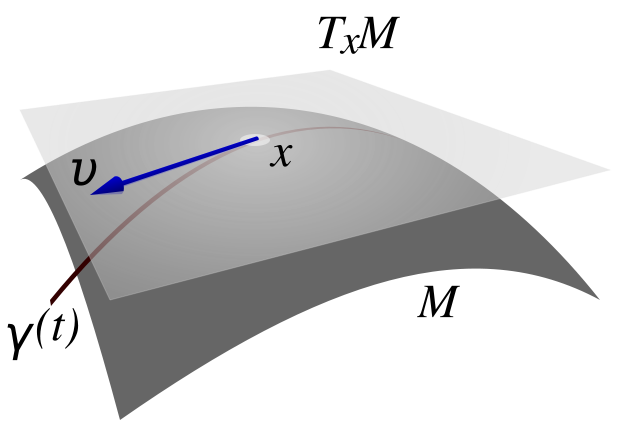
\includegraphics[width=7.0cm]{dev_tangentvec}
    \caption{方向微分と接ベクトル空間}
  \end{center}
\end{figure}


$\realnum^n$のときは$\delxkf(p)$達の値が分かっていれば,他の方向に関する微分はそれらの線形結合で表せたが,$S^2$のときはいちいち対応する曲線を求めなくてはいけないのだろうか.ここで,最初に考えていた,局所座標$(\varphi_{x\pm};U_{x\pm}),(\varphi_{y\pm};U_{y\pm}),(\varphi_{z\pm};U_{z\pm})$達が役に立つのである.今,$p$は$U_{x+}$に入っていることから,$\varphi_{x+}^{-1}$によって$q=(\frac{1}{\sqrt{3}},\frac{1}{\sqrt{3}})\in V_{x+}$に移る.$\gamma$を$t=0$で$p$を通る曲線とする.$\gamma$(の$U_{x+}$に入っている部分)を$\varphi_{x+}^{-1}$によって$V_{x+}$に移すと,$V_{x+}$上の曲線$\tilde{\gamma}$が得られる.このとき,$\tilde{\gamma}(0)=q$であり,$\dfrac{d\tilde{\gamma}}{dt}\Big|_{t=0}=(b_1,b_2)$とおくと,今$f\circ \varphi_{x+}$の定義域は$\realnum^2$の開集合であるから,先程の議論より$f\circ\varphi_{x+}$の$\tilde{\gamma}$方向の微分は$\dfrac{\partial (f\circ\varphi_{x+})}{\partial y}(q)b_1+\dfrac{\partial (f\circ\varphi_{x+})}{\partial z}(q)b_2$と表せる.ここで,$f\circ \varphi_{x+}$の$\tilde{\gamma}$方向の微分は$\dfrac{d(f\circ\varphi_{x+}\circ\tilde{\gamma}(t))}{dt}\Big|_{t=0}=\dfrac{d(f\circ\varphi_{x+}\circ\varphi_{x+}^{-1}\circ\gamma(t))}{dt}\Big|_{t=0}=\dfrac{d(f\circ\gamma(t))}{dt}\Big|_{t=0}$となって,$f$の$\gamma$方向の微分と等しい.よって全ての方向の微分は$\dfrac{\partial (f\circ\varphi_{x+})}{\partial y}(q),\dfrac{\partial (f\circ\varphi_{x+})}{\partial z}(q)$の線形結合で与えられることが分かる.


しかしだからといって$f\circ \varphi_{x+}$のヤコビ行列$J_{f\circ \varphi_{x+}}$について,$J_{f\circ\varphi_{x+}}$倍写像$\realnum^2\rightarrow \realnum$そのものを$f$の微分とするのはいささか抵抗がある.というのも,$p$は$U_{y+},U_{z+}$上の点でもあるので,$\varphi_{x+}$との合成だけ特別扱いするのは変だからである.しかも,一般には$J_{f\circ\varphi_{x+}}\neq J_{f\circ\varphi_{y+}}$であるから,別の局所座標を取れば別のヤコビ行列が得られる.なぜこのようなことがおきるのかというと,これらの線形写像の定義域が局所座標の取り方に依存してしまうからである.では$p$における全ての「方向」の空間を局所座標に依らない形で定義するにはどうすればいいだろうか.$p$を通るような曲線$\gamma$について,$\gamma$方向の$f$の微分が考えられたので,そのような$\gamma$全体の集合を「方向」の集合とすればよいと思うかもしれないが,そのような集合は大きすぎて,その中で和やスカラー倍をどう定義するかは自明ではない.和やスカラー倍が定義されていない集合を定義域とする写像では,そもそも「線形写像」の概念を考えられない.


ここで,発想の転換を行う.今まで思い描いてきた理想像は,適当な関数$f$が与えられると,「$p$における方向全体の集合」から$\realnum$への線形写像が一つ定まるというものだった.これは,適当な関数$f$と$p$における方向を定めると,実数が定まるということにになる.すなわち見方を変えると,$p$における方向が与えられると,「微分可能な関数」全体から$\realnum$への写像が一つ定まるということになる.この「微分可能な関数」全体から$\realnum$への写像全体の部分集合として,「$p$における方向全体の集合」を定義してしまおう.微分をまだ定義していないのに「微分可能な関数」を定めるのは変な感じを受けるかもしれないが,局所座標を用いれば簡単に定義できる.「微分可能な関数」の集合$C^\infty(S^2)$を次のように定める.$f:S^2\rightarrow \realnum$が$C^{\infty}$級であるとは,任意の$p\in S^2$に対して$p$が入るような局所座標$(\varphi;U)$を1つ取った時,$f\circ\varphi:\varphi^{-1}(U)\rightarrow \realnum$が$\varphi^{-1}(p)$で$C^{\infty}$級\footnote{つまり,任意の自然数$n,m$に対して,$\dfrac{\partial^{n+m}f}{\partial x_1^n\partial x_2^m}$が存在するということ.}であることをいい,$C^\infty$級の関数全体を$C^\infty(S^2)$で表す.


今,$C^{\infty}(S^2)$から$\realnum$への写像全体を$\mathcal F$と置くと,$\mathcal F$上には「和」と「($\realnum$による)スカラー倍」が定義される.具体的には,2つの${\mathcal F}$の元$D,D':C^{\infty}(S^2)\rightarrow \realnum$と$\lambda\in\realnum$に対して,$\lambda D,D+D'\in{\mathcal F}$を任意の$f\in C^{\infty}$に対し$(\lambda D)(f)=\lambda(D(f)),(D+D')(f)=D(f)+D'(f)$と定めればよい.このように「和」と「($\realnum$による)スカラー倍」が定義されていて,結合法則などのいくつかの良い性質を満たす集合を,「$\realnum$線形空間\footnote{$\realnum$が明らかなときはしばしば省略される.}」という.さて,$\delyp,\delzp$という$\mathcal F$の元を,
$$
\delyp:f\mapsto \dfrac{\partial (f\circ\varphi_{x+})}{\partial y}(\varphi_{x+}^{-1}(p))\quad
\delzp:f\mapsto \dfrac{\partial (f\circ\varphi_{x+})}{\partial z}(\varphi_{x+}^{-1}(p))
$$
と定め,これらの線形結合で表されるような$\mathcal F$の元,すなわちある$b_1,b_2\in\realnum$を用いて$b_1\delyp+b_2\delzp$と書けるような元全体を$T_pS^2$とおく.この集合は定義から「和」と「スカラー倍」について閉じている.すなわち,任意の$D,D'\in T_pS^2$および$\lambda\in\realnum$に対し,$\lambda D,D+D'\in T_pS^2$となる.このような線形空間の部分集合を「部分空間」という.線形空間の部分空間はそれ自身が線形空間になっている.$T_pS^2$は$S^2$における「接ベクトル空間」と呼ばれる.


いきなり天下り的に接ベクトル空間$T_pS^2$というものが導入されてしまったが,これこそが求めていた$p$における「方向」全体の集合になっている.というのも,$\gamma(0)=p$を満たす曲線$\gamma$について,$\gamma$の方向微分$D_\gamma:C^{\infty}(S^2)\rightarrow\realnum$は$D_\gamma(f)=\dfrac{d(f\circ\gamma(t))}{dt}\Big|_{t=0}$で与えられたのだったが,これは結局$\gamma$を局所座標$(\varphi_{x+};U)$によって$V_{x+}$上の曲線$\tilde{\gamma}$とみることによって,$\dfrac{d\tilde{\gamma}}{dt}\Big|_{t=0}=(b_1,b_2)$とおくと,
$$D_\gamma(f)=\dfrac{d(f\circ\varphi_{x+}\circ\tilde{\gamma}(t))}{dt}\Big|_{t=0}=\dfrac{\partial (f\circ\varphi_{x+})}{\partial y}(\varphi_{x+}^{-1}(p))b_1+\dfrac{\partial (f\circ\varphi_{x+})}{\partial z}(\varphi_{x+}^{-1}(p))b_2=\left(b_1\delyp+b_2\delzp\right)(f)
$$
となって$D_{\gamma}\in T_pS^2$がわかり,逆に,任意の$b_1,b_2\in\realnum$に対して,$b=\tenchi(b_1,b_2)$とし,$\realnum^2$の曲線$\tilde{\gamma'}:\realnum\rightarrow\realnum^2$を$\tilde{\gamma'}(t)=\varphi_{x+}^{-1}(p)+tb$で定め,$V_{x+}$に入っている部分を$\varphi_{x+}$によって$S^2$上に送った曲線を$\gamma'$と置くと,$\gamma'$の方向微分$D_{\gamma'}$は$b_1\delyp+b_2\delzp$となる.よって$p$における任意の「方向」は$T_pS^2$の元として表され,$T_pS^2$の任意の元は$p$における方向を表すので$T_pS^2$は$p$における「方向」全体の集合と見なせる.$p$における「方向」は,すなわち,$p$における$S^2$の接平面を表していると考えることもできるため,「接ベクトル空間」という名前になっているのである.



ここで一つ注意したいのが,$T_pS^2$は定義の際に局所座標$(\varphi_{x+};U_{x+})$を使っているが,実は局所座標の取り方によらない.例えば,別の局所座標$(\varphi_{y+};U_{y+})$を取ってみよう.このとき,
$$
\delxp':f\mapsto \dfrac{\partial (f\circ\varphi_{y+})}{\partial x}(\varphi_{y+}^{-1}(p))\quad
\delzp':f\mapsto \dfrac{\partial (f\circ\varphi_{y+})}{\partial z}(\varphi_{y+}^{-1}(p))
$$
という2つの$\mathcal F$の元がそれぞれ$T_pS^2$に入っていることを示せば,$\delxp',\delyp'$の線形結合で表されるような元全体$A$が$T_pS^2$に含まれていることが示せ,対称性より逆に$T_pS^2$が$A$に含まれていることが分かり,結局$T_pS^2=A$となって局所座標の取り方に依らない.今,$\varphi_{x+}^{-1}\circ\varphi_{y+}:\varphi_{y+}^{-1}(U_{x+}\cap U_{y+})\rightarrow\varphi_{x+}^{-1}(U_{x+}\cap U_{y+})$が$\realnum^2$の開集合から$\realnum^2$の開集合への写像になっていることを考えると,1章における連鎖律からら,$J_{f\circ\varphi_{y+}}=J_{f\circ\varphi_{x+}}J_{\varphi_{x+}^{-1}\circ\varphi_{y+}}$となる.ここで$J_{\varphi_{x+}^{-1}\circ\varphi_{y+}}$は$f$に依らないから,$J_{\varphi_{x+}^{-1}\circ\varphi_{y+}}=\vecb c_{11} && c_{12} \\ c_{21} && c_{22}\vece$とおくと,上の式は,
$$
\left(\delxp'(f)\quad\delzp'(f)\right)=\left(\delyp(f)\quad\delzp(f)\right)\vecb c_{11} && c_{12} \\ c_{21} && c_{22}\vece
$$
となる.任意の$f$について上の式は成り立つから,$\mathcal F$の元として
$$
\left(\delxp'\quad\delzp'\right)=\left(\delyp\quad\delzp\right)\vecb c_{11} && c_{12} \\ c_{21} && c_{22}\vece
$$
が成り立つので,各成分を比較すれば,$\delxp',\delzp'$が$T_pS^2$に入っていることが示される.


\Subsection{微分写像とrank}
さて,前節では苦労を重ねて$p$における$S^2$の方向の集合$T_pS^2$が局所座標に依らない形で定義出来たわけだが,ここまで定義されれば$f\in C^{\infty}(S^2)$の$p$における微分は簡単に定義できる.$D\in T_pS^2$の元に対して,$D(f)\in \realnum$を対応させる写像を$(df)_p:T_pS^2\rightarrow \realnum$とあらわし,$f$の$p$における微分写像という.これは定義から線形写像,すなわち任意の$\lambda\in\realnum, D,D'\in T_pS^2$に対して,$(df)_p(\lambda D)=\lambda (df_p)(D)$および$(df)_p(D+D')=(df)_p(D)+(df)_p(D')$が成り立っていることがすぐわかる.しかし,$(df)_p$は抽象的な空間から$\realnum$への線形写像なので,どのような写像なのかよくわからない.ここで,線形空間を理解するための一つのツールとして,「基底」というものを導入しよう.$T_pS^2$の元は$b_1,b_2\in\realnum$を用いて$b_1\delyp+b_2\delzp$とあらわされているのだった.もし,この表示が一意的ならば,$\realnum^2$から$T_pS^2$への写像
$(b_1,b_2)\mapsto b_1\delyp+b_2\delzp$が全単射線形写像となり,$T_pS^2$は$\realnum^2$と線形空間として「同型」,すなわちこの基底を介して,$\realnum^2$と$T_pS^2$は同じものと見なせる.さて,$b_1\delyp+b_2\delzp$という表示が一意的かどうか確かめるためには,$b_1\delyp+b_2\delzp=0$となる$b_1,b_2$が$(b_1,b_2)=(0,0)$のみ,すなわち$\delyp$と$\delzp$が1次独立であることを確かめればよい.$b_1\delyp+b_2\delzp=0$とする.これは$\mathcal F$における等式だから,すなわち任意の$f\in C^{\infty}(S^2)$に対して$b_1\delyp(f)+b_2\delzp(f)=0$となる.このとき$f,g\in C^{\infty}(S^2)$として$f(x,y,z)=y,g(x,y,z)=z$を取れば,$\delyp(f)=1,\delzp(f)=0$より$b_1=0$で,$\delyp(g)=0,\delzp(g)=1$より$b_2=0$となって,$\delyp,\delzp$が1次独立であることがわかった.

\begin{figure}[h]
  \begin{center} 
    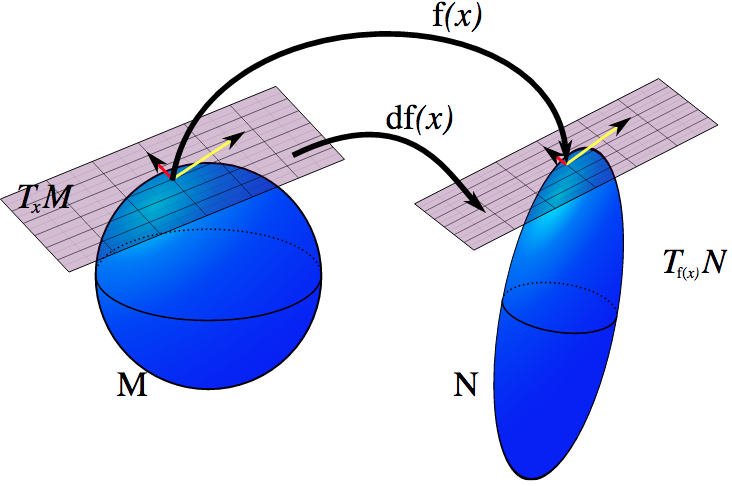
\includegraphics[width=7.0cm]{dev_diff}
    \caption{接ベクトル空間と微分写像}
  \end{center}
\end{figure}

この全単射同型写像$\realnum^2\rightarrow T_pS^2$と$(df)_p:T_pS^2\rightarrow \realnum$の合成は$\realnum^2$から$\realnum$への線形写像なので行列$P$で表されるはずだが,どのような行列なのだろうか.実は$P$は既に登場していた$J_{f\circ\varphi_{x+}}$に他ならない.というのも,$P$の第1列は$\delyp(f)=\dfrac{\partial (f\circ\varphi_{x+})}{\partial y}(\varphi_{x+}^{-1}(p))=J_{f\circ\varphi_{x+}}\vecb 1 \\ 0\vece$にほかならず,第2列も$\delzp(f)=\dfrac{\partial (f\circ\varphi_{x+})}{\partial z}(\varphi_{x+}^{-1}(p))=J_{f\circ\varphi_{x+}}\vecb 0 \\ 1 \vece$となって,結局$P$と$J_{f\circ\varphi_{x+}}$は一致する.重ね重ねになってしまうが,基底$\delyp,\delzp$による$(df)_p$の表示が$J_{f\circ\varphi_{x+}}$であるだけで,$(df)_p$そのものと$J_{f\circ\varphi_{x+}}$は違う.現に別の基底$\delxp',\delzp'$をとると行列表示は$J_{f\circ\varphi_{y+}}$へと変化する.有限次元\footnote{ある自然数$n$が存在して,$n$個以上の元が必ず1次従属になってしまうような線形空間.}の$\realnum$線形空間は「基底を取れば」,ある自然数$n$を用いて$\realnum^n$と線形空間として同型になるので,一見するとすべて線形空間は$\realnum^n$としてよく,抽象的な線形空間を導入する意義はないように思えるが,しかし,今回の$T_pS^2$のように「標準的な」基底がとれない場合もあり,そういう場合に抽象的な線形空間論が役に立つのである.実際に計算する段階では基底をとって具体的な行列やベクトルの計算に帰着させることができ,理論を考える際には抽象的な線形空間で考えることができるのが線形空間論の醍醐味であると思う.


話題が横道にそれてしまった.基底をとると$(df)_p$が$J_{f\circ\varphi_{x+}}$で表されるということは,基底を変えても変わらないような$J_{f\circ\varphi_{x+}}$の不変量は$(df)_p$に固有のものと考えてよい.このような不変量の代表的なものに,線形写像のrankの概念がある.行列のrankの概念を思い出そう.$m$行$n$列の行列$A$に対して,正則な$m$次正方行列$P$および正則な$n$次正方行列$Q$が存在して,
$$
PAQ=\vecb E_r && 0 \\ 0 && 0 \vece
$$
と一意的にあらわされるのだった.ここで$r$は$0\le r \le \min\{m,n\}$を満たす整数であり,$E_r$は$r$次の正方行列を表す.この$r$を行列$A$のrankという.左右から掛けられている$P,Q$は$\realnum^m,\realnum^n$における基底の取り換えを表していたのだったから,そもそもrankという概念は基底の取り換えによって不変,すなわち線形写像に固有の値である.線形写像のrankは,線形写像による像\footnote{一般に,線形空間$W,W'$および,線形写像$g:W\rightarrow W'$が与えられたとき,$g$による$W$の像$g(W)$は$W'$の部分空間となっている.}が値域の中で何次元\footnote{線形空間について,1次独立な元の最大個数を次元という.}の部分空間になっているかを示すものである.具体例を見てみよう.$f:S^2\rightarrow\realnum;(x,y,z)\mapsto c$(定値写像)および$g:S^2\rightarrow\realnum;(x,y,z)\mapsto x$という2つの写像の$p=(\frac{1}{\sqrt{3}},\frac{1}{\sqrt{3}},\frac{1}{\sqrt{3}})$における微分写像$(df)_p,(dg)_p$を考える.計算する前にそれぞれの微分写像のrankを予想してみよう.前者は$\realnum$において像が1点につぶれているから,$S^2$の任意の方向は0に潰れてしまう.よって微分写像の像の次元は0次元で$\rank(df)_p=0$となるだろう.一方,後者は像が$\realnum$において広がりを持っているから,$S^2$の方向は潰れずにのこり,微分写像のrankは$\rank(dg)_p=1$となるだろう.実際,
$$
\rank(df)_p=\rank J_{f\circ\varphi_{x+}}=\rank(0\:\:0)=0,\quad\rank(dg)_p=\rank J_{g\circ\varphi_{x+}}=\rank(-1\:\:-1)=1
$$
となる.


ここで例が$S^2$だけだと寂しいので,一般の多様体の概念を導入しておこう(上手くイメージ出来なかったら,$S^2$のように$\realnum^n$の開集合がペタペタはり合わされているような図形と考えればよい).
\begin{figure}[h]
  \begin{center} 
    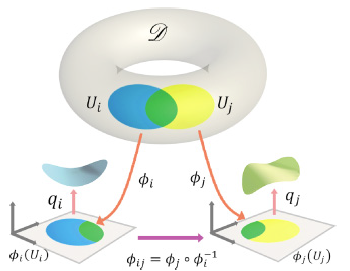
\includegraphics[width=7.0cm]{dev_manifold}
    \caption{多様体のイメージ}
  \end{center}
\end{figure}

\begin{s_defi}
$\realnum^l$の部分集合$M$が$n$次元の($C^\infty$級)\textbf{多様体}であるとは,
$M$が$M$の開集合の集まり$\{U_i\}_{i\in I}$で覆われていて,
かつ各$i$に対して$\realnum^n$の開集合$V_i$および同相写像$\varphi_i:V_i\rightarrow U_i$が存在することをいう.
さらに,$(\varphi_i;U_i)$の組は座標近傍と呼ばれ,
$U_i\cap U_j\neq \emptyset$のとき,
$\varphi_i^{-1}\circ\varphi_j:\varphi_j^{-1}(U_i\cap U_j)\rightarrow\varphi_i^{-1}(U_i\cap U_j)$が$C^{\infty}$級であるする.
\end{s_defi}



このとき,前節と同様にして,$M$上の$C^{\infty}$級関数の集合$C^{\infty}(M)$は,各点において座標近傍$\varphi_i$との合成が$C^{\infty}$級であるような関数の集合とし,$C^{\infty}(M)$から$\realnum$への写像全体がなす線形空間を${\mathcal F}(M)$とおく.$p\in M$が入るような座標近傍$(\varphi_i;U_i)$について,$V_i$における座標を$x_1,\dots,x_n$とすると$\delxop,\dots,\delxnp$というような$n$個の方向微分が考えられ,これらの1次結合によってあらわされるような${\mathcal F}(M)$の部分空間を$T_pM$とあらわし,$M$の$p$における接ベクトル空間という.この節のはじめに示したのと(だいたい)同じような方法で$\delxop,\dots,\delxnp$が1次独立であることが示せ,$T_pM$は$n$次元線形空間となる.\par


多様体の例としては,$\realnum^n$や$S^{n-1}=\{(x_1,\dots,x_n)\in\realnum^n|x_1^2+\dots+x_n^2=1\}$(これは$n-1$次元の多様体である)といった代表的なものを考えればこの記事の中では十分である.さて,$f:M\rightarrow N$を多様体の間の写像とする.$f$が$C^{\infty}$級とは,$M$の各点$p$において,$p$の座標近傍$(\varphi;U)$および$f(p)$の座標近傍$(\psi;U')$が存在して,$\psi^{-1}\circ f\circ\varphi$が$C^{\infty}$級であることを言う.さて,$f$が$C^{\infty}$級のとき,$M$の各点$p$において微分写像$(df)_p:T_pM\rightarrow T_{f(p)}N$が次のように定義される.まず,前章と同じようにして,$T_pM$の任意の元は$\gamma(0)=p$を満たす$M$上の曲線$\gamma$を用いて$D_\gamma(\gamma の方向微分)$と書けることが示せる.ただし,$D_\gamma$は$h\in C^\infty(M)$に対して,$\dfrac{d(h\circ\gamma(t))}{dt}\Big|_{t=0}$を返す写像である.$f\circ\gamma$は$f\circ\gamma(0)=f(p)$を満たす$N$上の曲線となる.$f\circ\gamma$方向の微分$D_{f\circ\gamma}\in T_{f(p)}N$を考え,$D_{\gamma}\mapsto D_{f\circ\gamma}$によって$(df)_p$を定める.\footnote{本来なら,これが$\gamma$の取り方によらないで定まることをしめす必要があるが,座標近傍を取ってみればわかることなので,ここでは省略した}なお,$p$の座標近傍$(\varphi;U)$および$f(p)$の座標近傍$(\psi;U')$を1つとり,$U$での$T_pM$の基底を$\delxop,\dots,\delxnp$,$U'$での$T_{f(p)}N$の基底を$\delyofp,\dots,\delymfp$とすると,これらの基底に関する$(df)_p$の行列表示は$J_{\psi^{-1}\circ f\circ\varphi}$で与えられる.


さて,一般の多様体を導入したのは,次の定理の説明をしたかったらである.
\begin{s_theo}
$f:M\rightarrow N$を多様体の間の$C^\infty$級写像で,$M$の次元$m$と$N$の次元$n$が$m\ge n$を満たしているとする.$q\in N$が正則値,すなわち,任意の$p\in f^{-1}(q)$について,微分写像$(df)_p$のrankが$n$であるとする.このとき,$f^{-1}(q)$は$m-n$次元の$C^{\infty}$級多様体となる.
\end{s_theo}
まず,この定理を応用すれば様々な多様体の例が得られることに注目してみよう.例えば,$f:\realnum^4 \rightarrow \realnum;(x,y,z,w)\mapsto x^2+y^2+z^2+w^2$という写像と,$1\in \realnum$について上の定理を適用してみると,$\rank(df)_p=\rank J_{f}=\rank(2x\:2y\:2z\:2w)\neq 0 (なぜなら(x,y,z,w)\in f^{-1}(1)よりx,y,z,wのいずれかは0でない)$より$x^2+y^2+z^2+w^2=1$で表される$\realnum^4$の部分集合(3次元球面)が,3次元多様体となることの証明が得られる.他にも,例えば$f:\realnum^3\rightarrow \realnum;(x,y,z)=x^2+y^2-z^2$と$-1\in\realnum$に適用して,2葉双曲面が2次元多様体になることもわかる.
この定理のイメージを述べよう.線形写像のrankは上で見たように,像が値域の中で何次元になっているかを表している.$(df)_p$のrankが$n$,すなわち$T_pN$の次元に等しいということは,それぞれの基底をうまく選ぶことによって,$(df)_p$は$(E_n\:\:0)$と行列表示できるということだから,このうまく選んだ$T_pM$の基底$D_1,\dots,D_m$について,$D_1,\dots D_n$という方向は$f$によって保たれ,残りの$D_{n+1},\dots,D_m$という方向は$f$によってつぶれるということがわかる.この$m-n$個の元がなす$T_pM$の部分空間は,$M$における$f$の等位面$f^{-1}(q)$の接空間とみなせる.接空間が$m-n$次元になっているため,$p\in f^{-1}(q)$の十分近くでは$\realnum^{m-n}$の開集合と同相と見なせて,結局$m-n$次元の多様体とみなせる.なお,この定理においてrankの条件は本質的であり,例えば$f:\realnum^2\rightarrow\realnum;(x,y)\mapsto y^2-x^2(x+1)$という写像を考えると,点$(0,0)\in\realnum^2$でヤコビ行列が0になるため,上の定理からは$f^{-1}(0)$は1次元多様体になるかわからない.実際,$f^{-1}(0)$は$(0,0)$の近傍においては2つの曲線が交わる形になっていて,$\realnum$のどんな開集合(すなわち開区間)と同相ではないので1次元多様体とはならない.


\Subsection{ベクトル場と積分曲線}
接ベクトル空間を導入したので,最後に応用のひとつとして多様体上のベクトル場を考えよう.$M$を$m$次元多様体とする.このとき,$M$の各点$p$に対して,$p$の周りの方向全体の空間,接ベクトル空間$T_pM$が定まっているのであった.各$p$に対して,$T_pM$の元を対応させる対応を「ベクトル場」という.今ベクトル場を$X$と言った時には,$X(p)$で$p$が指定する$T_pM$の元を表すことにする.例えば2次元多様体$\realnum^2$のベクトル場を考えよう.このとき,局所座標として$\realnum^2$から$\realnum^2$への恒等写像$(x,y)\mapsto (x,y))$が考えられる(したがって,この場合は「局所」座標が大域座標になっている).$\realnum^2$の接ベクトル空間$T_p\realnum^2$は$\delxp,\delyp$で張られる2次元の線形空間になっている.例えば,$X(p)=-y\delxp+x\delyp$というようなベクトル場が与えられたとしよう.これはより古典的な見方をすると,点$(x,y)$に対してベクトル$\tenchi(-y,x)$が対応しているようなベクトル場と考えることが出来る.試しに$xy$平面上のいくつかの点でベクトルを矢印で表してみると,原点を中心にぐるぐる時計周りに矢印が回るような絵が描ける.


もう少し自明でない例として球面$S^2$上のベクトル場を考えよう.この場合は一つの大域的な座標があるわけではないので,上のように明示的な表示を得るためには各点が含まれる座標近傍で指定する必要がある.座標近傍の組は前の前の章で考えたものを使うことにしよう.
\begin{eqnarray*}
p\in U_{x+}ならX(p) & = &\sqrt{1-y^2-z^2}\delyp \\
p\in U_{x-}ならX(p) & = &-\sqrt{1-y^2-z^2}\delyp  \\
p\in U_{y+}ならX(p) & = &-\sqrt{1-x^2-z^2}\delxp \\
p\in U_{y-}ならX(p) & = &\sqrt{1-x^2-z^2}\delxp \\
p\in U_{z+}ならX(p) & =  &-y\delxp+x\delxp \\
p\in U_{z-}ならX(p) & = &-y\delxp+x\delxp 
\end{eqnarray*}
とそれぞれ定める.これがきちんと定義されていること(well-defined)であることを確認する必要がある.たとえば,$p\in U_{y+}\cap U_{z+}$のとき,上で定めている$X(p)$が同じものを示しているかを確認しなくてはならない.このケースだけ確認してみよう.今紛らわしいので$U_{z+}$の方の座標は$(x',y')$であらわすことにしよう,したがって$U_{z+}$における$T_PS^2$の基底は$\delxdp,\delydp$とあらわすことにしよう.$\delxp,\delzp$と$\delxdp,\delydp$の関係は$\varphi_{z+}^{-1}\circ\varphi_{y+}:\varphi_{y+}^{-1}(U_{y+}\cap U_{z+})\rightarrow\varphi_{z+}^{-1}(U_{y+}\cap U_{z+})$のヤコビ行列$J_{\varphi_{z+}^{-1}\circ\varphi_{y+}}$を用いて
$$
\left(\delxp\quad\delzp\right)=\left(\delxdp\quad\delydp\right)J_{\varphi_{z+}^{-1}\circ\varphi_{y+}}
$$
と書けるのであった(1節の終わり参照).$J_{\varphi_{z+}^{-1}\circ\varphi_{y+}}$の各成分を具体的に計算してみよう.$\varphi_{z+}^{-1}\circ\varphi_{y+}$は$(x,z)\mapsto(x,\sqrt{1-x^2-z^2},z)\mapsto(x,\sqrt{1-x^2-z^2})$と書けるから,$x'=x,y'=\sqrt{1-x^2-z^2}$であり,ヤコビ行列は
$$
\vecb
1 && 0 \\
\frac{-x}{\sqrt{1-x^2-z^2}} && \frac{-z}{\sqrt{1-x^2-z^2}}
\vece
$$
となって,$\delxp=\delxdp+\dfrac{-x}{\sqrt{1-x^2-z^2}}\delydp$がわかる.よって$-\sqrt{1-x^2-z^2}\delxp =-\sqrt{1-x^2-z^2}\left(\delxdp+\dfrac{-x}{\sqrt{1-x^2-z^2}}\delydp\right) =-y'\delxdp+x'\delydp$となって$U_{y+}$での表示と$U_{z+}$での表示が一致することが確かめられる.


しかし,上のベクトル場$X$がどのようなベクトル場になっているのか上の表示だけから推察するのは容易ではない.そこで,もうすこしわかりやすく表すことを考えよう.包含写像$i:S^2\rightarrow\realnum^3$を考える.このとき,各$p$において微分写像$(di)_p:T_pS^2\rightarrow T_p\realnum^3$が考えられる.このとき,$(di)_p$は単射であることが次のようにわかる.$T_pS^2$の任意の元は$p$を通る曲線$\gamma$を用いて$D_\gamma$と書けたことを思い出そう.$\gamma,\gamma'$を$t=0$で$p$を通る曲線として$D_\gamma,D_{\gamma'}\in T_pS^2$について,$(di)_p(D_\gamma)=(di)_p(D_{\gamma'})$となったとしよう.すると,定義より$D_{i\circ\gamma}=D_{i\circ\gamma}$だから,任意の$C^\infty(\realnum^3)$の元(これは単なる$\realnum^3$上の$C^\infty$級関数)$f$に対して$\dfrac{d(f\circ i\circ\gamma(t))}{dt}\Big|_{t=0}=\dfrac{d(f\circ i\circ\gamma'(t))}{dt}\Big|_{t=0}$となる.今例えば$f$として,$f(x,y,z)=x,f(x,y,z)=y,f(x,y,z)=z$を代入してみると,$\dfrac{d\gamma}{dt}\Big|_{t=0}$と$\dfrac{d\gamma'}{dt}\Big|_{t=0}$の$x$成分,$y$成分,$z$成分が一致することが確かめられて,$\dfrac{d\gamma}{dt}\Big|_{t=0}$=$\dfrac{d\gamma'}{dt}\Big|_{t=0}$がわかり,$\realnum^3$内で考えたとき2つの曲線$\gamma,\gamma'$の$p$における接ベクトルは等しい.よって$T_pS^2$の元としても$D_\gamma$と$D_{\gamma'}$は一致することがわかる.


一般に,線形空間$W,W'$および,単射線形写像$g:W\rightarrow W'$が与えられたとき,$g(W)$は$W$と同型な線形空間になる.上の$(di)_p$によって,$T_pS^2$は$T_p\realnum^3$の部分空間と同一視できる.さて,ベクトル場$X$は$p$に$X(p)\in T_pS^2$を対応させる写像だったが,$X(p)$の元を$(di)_p$によって$T_p\realnum^3$に送ってみよう.$T_p\realnum^2$のときと同じように,3次元多様体には大域的な局所座標$x,y,z$が存在する.今球面上の局所座標と区別するため,$\realnum^3$の局所座標は$x',y',z'$と書くことにする\footnote{上の$x',y'$とは何の関係もない.}と,$T_p\realnum^3$は$\delxdp,\delydp,\delzdp$で張られる3次元線形空間である.$i:S^2\rightarrow\realnum^3$は例えば,局所座標$(\varphi_{x+};U_{x+})$を使って表示すると,$(y,z)\mapsto(\sqrt{1-y^2-z^2},y,z)$であるから,$\delyp,\delzp$と$\delxdp,\delydp,\delzdp$との関係は,$i\circ\varphi_{x+}$のヤコビ行列を考えて,
$$
\left(\delyp\quad\delzp\right)=\left(\delxdp\quad\delydp\quad\delzdp\right)
\vecb
\frac{-y}{\sqrt{1-y^2-z^2}} && \frac{-z}{\sqrt{1-y^2-z^2}} \\
1 && 0 \\
0 && 1
\vece
$$
となる.よって,$X(p)=\sqrt{1-y^2-z^2}\delyp=-y\delxdp+\sqrt{1-y^2-z^2}\delydp=-y'\delxdp+x'\delydp$と表示できる.他の座標近傍に関しても同様の表示が出来ることを確かめると,結局$\realnum^3$の中で考えると各$(x,y,z)$に対して$\tenchi(-y,x,0)$というベクトルが対応するようなベクトル場と考えることが出来る.すなわち,右手系\footnote{$x$軸方向を右手の親指,$y$軸方向を人差し指,$z$軸方向を中指に対応させるような座標系の取り方}で考えれば,$(0,0,1)$を北極として各点で東の方向に大きさ$\sqrt{x^2+z^2}$の矢印が向いているような絵が描けるだろう.ベクトル場を風に例えるなら,低緯度ほど強い東向きの風が吹いていて,高緯度につれて弱くなっているようなイメージが出来る.ところで,各点において,ベクトル$\tenchi(-y,x,0)$はベクトル$\tenchi(x,y,z)$,すなわち各点の位置ベクトルと直交していることに注目してみる.さらに言えば,上の記号を使えば$(di)_p(\delyp),(di)_p(\delzp)$の表すベクトル$\tenchi(\frac{-y}{\sqrt{1-y^2-z^2}},1,0)$および$\tenchi(\frac{-z}{\sqrt{1-y^2-z^2}},0,1)$と$\tenchi(x,y,z)$は直交している.$T_pS^2$は$\delyp,\delzp$で生成されていたから,これは$(di)_p(T_pS^2)$が$S^2$に接していることを示しており,$T_pS^2$が「接」ベクトル空間を表していることの根拠のひとつと言えるだろう.


さて,例を見たところで一般の多様体$M$上のベクトル場$X$についてもう少し考えてみよう.$X$は一見すると写像に見えるが,$p\in M$ごとに行先の空間$T_pM$は異なるため,このままでは写像とはならないため,連続性などは定義出来ない.しかし,ベクトル場とみるときはある程度の「連続性」や「微分可能性」を仮定したくなる.つまり,$p,q\in M$が十分近ければ,$X(p),X(q)$もある程度「近く」あってほしい.ここで,$p\in M$が入るような局所座標$(\varphi_i:U_i)$において,$\varphi_i^{-1}(U)$における座標を$x_1\dots x_n$とすると,$T_pM$元は$\delxkp$達の線形結合$b_1(p)\delxop+\dots+b_n(p)\delxnp$(ただし,$b_k(p)\in \realnum$は$\delxkp$の係数である)と一意的に書けていたことに注目する.おなじ局所座標に入るような十分近い点$p,q\in M$については,この対応$p\mapsto b_k(p)$が「連続」や「微分可能」であることを$X$に要請すればよいことがわかる.より正確に(そして抽象的に)述べると次のようになる.

\begin{s_defi}
各点$p\in M$における接ベクトル空間$T_pM$を全て束ねたような空間を$TM=\coprod_{p\in M}T_pM$
\footnote{一般に,集合の集まり$\{A_i\}_{i\in I}$が与えられたとき,$\coprod_{i\in I}A_i$は任意の$i\neq j\in I$に対して$A_i\cap A_j=\emptyset$となるように和集合をとったものを表す.}と表し,\textbf{接ベクトルバンドル}という.
$TM$の元は$M$上の各点とその上の接ベクトル空間上の元の組と考えられるので,$T_pM\subset TM$の元を$p\in M$に対応させるような写像$\pi:TM\rightarrow M$を考えることが出来る.
このとき,$TM$は$\realnum^{2n}$の開集合と同一視できる空間$\{\pi^{-1}(U_i)\}_{i\in I}$によって覆われて,$2m$次元の多様体とみなせる.
ここで,ベクトル場$X$とは,多様体の写像$X:M\rightarrow TM$であって,任意の$p\in M$に対して$\pi\circ X(p) = p$を満たすものとして定義される.この写像が$C^{\infty}$級のときベクトル場$X$は$C^{\infty}$級と呼ばれる.
\end{s_defi}
\begin{Proof}
$TM$が$2m$次元の多様体の多様体になることについて証明する.\\
ここで,$M$の局所座標$(\varphi_i;U_i)$について,$\varphi_i^{-1}(U_i)$上の座標を$x_1\dots x_n$とする.$\pi^{-1}(U_i)\subset TM$の元は$2n$個の座標$x_1,\dots,x_n$($p$の座標を表す変数)および$b_1(p),\dots,b_n(p)$($\delxkp$の係数を表す変数)によって表示できるので,$\pi^{-1}(U_i)$は直積集合\footnote{一般に,$A$と$B$を集合として,直積集合$A\times B$は$A$の元と$B$の元の組全体の集合を表す.}$U_i\times \realnum^n$と考えることが出来る.つまり,全単射$\tilde{\varphi_i}:U_i\times \realnum^n\rightarrow\pi^{-1}(U_i);(x_1\dots,x_n,b_1,\dots,b_n)\mapsto ((x_1,\dots,x_n),b_1\delxop+\dots+b_n\delxnp)$によって,$\pi^{-1}(U_i)$の点は$U_i\times\realnum^n$と1対1に対応する.ここで,$U_i\times \realnum^n$は$\realnum^n\times \realnum^n$,すなわち$\realnum^{2n}$の開集合になっている.$\{(\varphi_i;U_i)\}_{i\in I}$を$M$の全ての局所座標とすると,$\{U_i\}_{i\in I}$は$M$を覆っていることから$TM$は$\realnum^{2n}$の開集合と同一視できる空間$\{\pi^{-1}(U_i)\}_{i\in I}$によって覆われるので,$2m$次元の多様体\footnote{注意深い人は,前節で定義した「多様体」は$\realnum^l$の部分集合になっていたので,$TM$が「多様体」となるためには$TM$がある$\realnum^l$の部分空間として表される必要があると考えるだろう.結果的にこのことは正しいが,ここではそれ以上触れない.}となる.今$\tilde{U_i}=\pi^{-1}(U_i)$と置くと.$\{(\tilde{\varphi_i};\tilde{U_i})\}_i$は$TM$の局所座標という.
\end{Proof}
さて,多様体$M$上の$C^\infty$級ベクトル場$X$が与えられたとき,ベクトル場に沿うような$M$上の曲線を積分曲線という.より正確に言いうと次のようになる.
\begin{s_defi}
$\realnum$の開区間$(a,b)$において定義された曲線$\gamma:(a,b)\rightarrow M$がベクトル場$X$の積分曲線であるとは,任意の$t\in(a,b)$について,$\gamma(t)$における$\gamma$の方向微分$D_\gamma\in T_{\gamma(t)}M$が$X(\gamma(t))$に一致することを言う.
\end{s_defi}
例えば,1番目の例であったら,原点を中心とする円$\gamma:\realnum\rightarrow \realnum^2;t\mapsto (\cos t,\sin t)$を考えると,各点での$\gamma$の接ベクトルは$\tenchi(-\sin t,\cos t)=(-y,x)$となってベクトル場と一致するので積分曲線になっているし,2番目の例でも,$\gamma:\realnum\rightarrow S^2;t\mapsto (\cos t,\sin t,0)$を考えれば同様に$\gamma$は積分曲線になっていることがわかる.

\begin{figure}[h]
  \begin{center} 
    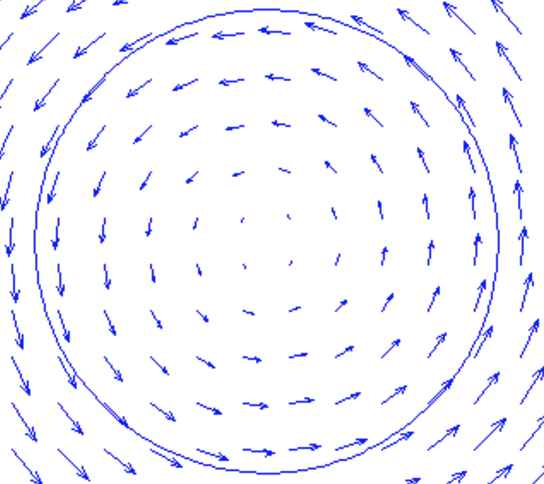
\includegraphics[width=7.0cm]{dev_vecfield}
    \caption{積分曲線の例}
  \end{center}
\end{figure}
さて,任意の点$p\in M$が与えられたとき,$t=0$で$p$を通るような積分曲線は存在するだろうか.十分小さい大きさの積分曲線に限って考えればこの事実は正しい.十分小さい範囲で考えれば,積分曲線は一つの局所座標の中に入っていると考えられるので,$p$が入るような局所座標$(\varphi;U)$を一つとる.$\varphi^{-1}(U)$における座標を$x_1\dots,x_n$として,ベクトル場$X$は$U$上で$n$個の$U$上の$C^\infty$級関数$b_1,\dots,b_n$を用いて$X\xvec=b_1\xvec\left(\dfrac{\partial}{\partial x_1}\right)_{\xvec}+\dots+b_n\xvec\left(\dfrac{\partial}{\partial x_n}\right)_{\xvec}$と表示されているとする.
求めたい$U$上の曲線$\gamma$は$n$個の未知関数$\gamma_1,\dots,\gamma_n$を用いて$\gamma(t)=(\gamma_1(t),\dots,\gamma_n(t))$と書けるから,$D_\gamma=X(\gamma(t))$という条件をこの局所座標上で書き直すと,初期条件が$\gamma(0)=p$で
$$
\frac{d\gamma_1(t)}{dt}\left(\dfrac{\partial}{\partial x_1}\right)_{\gamma(t)}+\dots+\frac{d\gamma_n(t)}{dt}\left(\dfrac{\partial}{\partial x_n}\right)_{\gamma(t)}
=b_1(\gamma(t))\left(\dfrac{\partial}{\partial x_1}\right)_{\gamma(t)}+\dots+b_n(\gamma(t))\left(\dfrac{\partial}{\partial x_n}\right)_{\gamma(t)}
$$
という微分方程式,すなわち,$\dfrac{d\gamma_i(t)}{dt}=b_i(\gamma_1(t),\dots,\gamma_i(t))\quad(1\le i\le n)$という1階の連立常微分方程式に帰着する.今各$b_i$が$C^\infty$級なので,常微分方程式の解の存在と一意性の定理から,ある$\varepsilon>0$が存在して,$\gamma(0)=p$を満たすような積分曲線$\gamma:(-\varepsilon,\varepsilon)\rightarrow M$が存在する.


しかし,この積分曲線必ずしも$\realnum$全体で定義された曲線$\gamma:\realnum\rightarrow M$に拡張するとは限らない.極端な例として,$M=\realnum^2-{(0,1)}$として,$M$上のベクトル場$X$を一番目の例と同じものとすると,$(1,0)$
からスタートした曲線が延長されるとすれば,先の常微分方程式の解の一意性より$\gamma:\realnum\rightarrow \realnum^2;t\mapsto (\cos t,\sin t)$に一致する必要があるが,$\gamma$は$(0,1)$を通れないので,結局$(0,1)$の手前までしか伸ばせず,$t=\frac{\pi}{2}$の手前で止まってしまう.このような状況がおきてしまうと,例えば積分曲線が何かの軌跡を表しているような状況を考えると,有限時間内までしかその物体を追えなかったり,軌跡から元の位置をさかのぼることが出来なくなったりするので困ったこととなる.このような困ったことが起きない,すなわち任意の積分曲線が$\realnum$全体まで延長できるようなベクトル場は「完備」であるといわれる.実は次の定理が成り立つ.
\begin{s_theo}
コンパクトな多様体上の任意の$C^\infty$級ベクトル場は完備である.
\end{s_theo}
よって,特に$n-1$次元球面はコンパクトなので,その上のベクトル場は完備となる.この定理の本質的な部分は,「コンパクト」という部分である.教養の解析学で習う基本的な定理として,「コンパクト集合における連続関数は最大値・最小値をもつ」という定理があった.上でのべたように,多様体の各点において$(-\varepsilon,\varepsilon)$で定義された積分曲線が存在する.このような$\varepsilon$の上限(ただし,上限が存在しない場合は適当な正数$R$をとるとする)を今$f(p)$とおこう.常微分方程式の解は初期値に連続に依存するので,$f$は連続.よって最小値をもつので,これを$\varepsilon_m$とおく.これは多様体の各点において$\varepsilon_m$だけ積分曲線を延長できることを示しているので,各点の積分曲線を繰り返し$\varepsilon_m$だけ伸ばしていくことで,$\realnum$全体で定義された積分曲線を得る.


さて,コンパクト多様体$M$上の完備なベクトル場が与えられたとき,$p\in M$に対して$t=0$で$p$を通るような$X$の積分曲線を$\gamma_p$とおく.$t\in\realnum$に対し,写像$F_t:M\rightarrow M$を$p\mapsto \gamma_p(t)$で定めよう.この写像は次の性質を満たす.
\begin{description}
\item{(1)} 任意の$p\in M$に対して,$F_0(p)=p$.
\item{(2)} 任意の$s,t\in\realnum$に対して,$F_s\circ F_t=F_{s+t}$
\end{description}
この$\{F_t\}_{t\in\realnum}$を\footnote{このように,あるパラメーターによって添え字づけられた集まりを$\{A_i\}_{i\in \Lambda}$のように書いたりする.たとえば,数列を$(a_n)_{n\in {\mathbb N}}$と書くのと気持ちは同じである.}ベクトル場$X$のフローという.性質(2)についてだが,これは任意の$p$において$\gamma_{\gamma_p(t)}(s)=\gamma_p(t+s)$を示せばよい.$\gamma':\realnum\rightarrow M;s\mapsto\gamma_p(s+t)$という曲線を考えよう.この曲線は$s=0$で$\gamma(t)$を通り,かつ元の積分曲線$\gamma_p$のパラメーターを平行移動させただけなので,積分曲線になっている.よって積分曲線の一意性から$\gamma_{\gamma_p(t)}$と一致する.なお,性質(2)から$F_t^{-1}=F_{-t}$となって,$F_t$は全単射であることがわかる.また,$F_t$が$C^\infty$級であることは次のようにわかる.まず,ある$T>0$が存在して,任意の$-T\le t\le T$に$F_t$が$C^\infty$級であることを示せばよい.なぜなら,任意の$t\in\realnum$に対して,$|t| \le nT$となる自然数$n$を選べば,性質(2)から$F_t$は$F_{\frac{t}{n}}$の$n$回合成として得られるので,$C^\infty$級である.今$T>0$は十分小さくできるので,$-T\le t \le T$のとき各点$p$に対して,$p$と$\gamma_p(t)$は同じ座標近傍に入るとしてよい.すると,$\realnum^n$の開集合のケースに帰着する.このときは常微分方程式の解は初期値に対して$C^\infty$級に依存するということが常微分方程式の理論からわかっているので,結局$F_t$は$C^\infty$級で,かつ逆写像も$C^\infty$級であることがわかる.ベクトル場のフローは,多様体上に「流れ」が与えられたときの時間経過と見なすことが出来る.たとえば,球面上のフローが海流を表しているとすると,時刻が$t$だけ経過したときに元の位置$p$からどれくらい流されているかの情報が$F_t$によって与えられる.


一方,上の性質を満たすような$C^\infty$級写像$F_t:M\rightarrow M$の集まり$\{F_t\}_{t\in\realnum}$であって,各$p\in M$に対して$F:\realnum\rightarrow M;t\mapsto F_t(p)$が$C^\infty$級であるものが与えられたとしよう.すると,$M$上の各点$p$に対して,$\gamma_p(t)=F_t(p)$によって$\gamma_p:\realnum\rightarrow M$を与えれば,$\gamma_p$は$M$上の曲線となる.$\gamma_p$は$t=0$で$p$を通るから,$M$上のベクトル場$X:p\mapsto D_{\gamma_p}$が定義でき,$F_t$が$C^\infty$級写像であることから$X$は$C^\infty$級ベクトル場であり,作り方から$\gamma_p$という積分曲線を各点で持つので完備である.以上のことから,コンパクト多様体上のベクトル場とフローの間には1対1の対応があり,一方が与えられれば,もう片方を構成できる.最後に$S^2$上の$C^\infty$級ベクトル場に関する興味深い事実を述べてこの記事を締めくくろうと思う.
\begin{s_theo}[ポアンカレ・ホップの定理の特別な場合]
$S^2$上の$C^\infty$級ベクトル場$X$は必ず零点,すなわち$X(p)=0$となる点を持つ
\end{s_theo}
この事実は,球面上生えている髪の毛をどのようにとかしてもつむじができてしまうという意味で"Hairly Ball Theorem"とも呼ばれる.今までの道具だけではこの定理の証明には立ち入ることが出来ないが,「オイラーの多面体公式」として知られている,(頂点の数)-(辺の数)+(面の数)=2の右辺が0でないことに起因するとだけ述べておこう.ところで,$S^2$はコンパクトなので,上の話からベクトル場とフローには1対1対応があったことを思い出そう.ベクトル場の零点となっているような点では,積分曲線がその点にとどまり続けるので,対応するフローの不動点となっている.今零点が必ず存在するということから,対応するフローには必ず不動点が存在する.逆に言えば不動点が存在しないような$C^\infty$級微分同相(逆写像が存在して$C^\infty$級ということ)$S^2\rightarrow S^2$は,フローのある時刻における写像$F_t:S^2\rightarrow S^2$として表されない.たとえば,$(x,y,z)\mapsto (-x,-y,-z)$という対蹠点に移す写像を考えると,不動点が存在しないので,どのような球面上のフロー$\{F_t\}_{t\in\realnum},t\in\realnum$についても$F_t$と一致しない.
\begin{figure}[h]
  \begin{center} 
    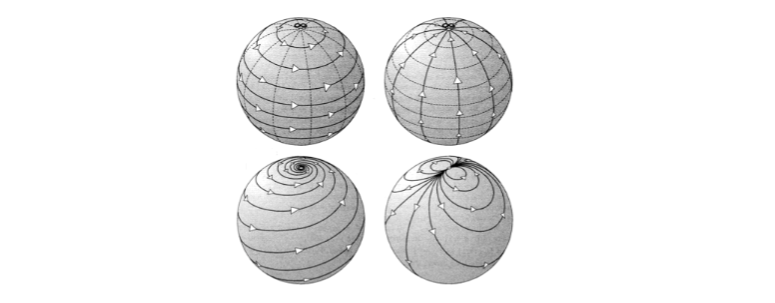
\includegraphics[width=9.0cm]{dev_phthm}
    \caption{ポアンカレ・ホップの定理の図}
  \end{center}
\end{figure}
\Section{あとがき}
「線形代数の広がり」といいつつ幾何的な話題に終始してしまったのはいささか申し訳ないという気持ちもあるが,自分が数学科に進学した後一番線形代数を使ったという印象を受けるのは多様体の講義だったのでこのテーマを選ばせていただいた.多様体の話は特に解析力学などを進んで学ぶ上では避けては通れないわりに,位相空間論を多少なりともやっていないと敷居が高いように感じてしまうので,この記事ではなるべく予備知識を仮定しないように努力したつもりである.特に以下の文献を参考にしたので,進んで学習する際には参考にすることをお勧めする.
\begin{thebibliography}{9}
\bibitem  杉浦光夫,『基礎数学3 解析入門 II』,東京大学出版会,1985
\bibitem  M. スピヴァック,『多変数解析学 古典理論への現代的アプローチ』,東京図書,1972
\bibitem  松本幸夫,『基礎数学5 多様体の基礎』,東京大学出版会,1988
\bibitem  J. W. ミルナー,『微分トポロジー講義』,丸善出版,2012
\bibitem  坪井俊,『幾何学I 多様体入門』,東京大学出版会,2005
\end{thebibliography}
最後にここまで読んでくださった読者のみなさん,そして編集者のすうさんに限りない感謝を述べて結びといたします.
